\documentclass[]{article}
\usepackage{graphicx}
\usepackage{caption}
\captionsetup{font={small}}   %% 这一句放在 caption前面


%opening
\title{Who are we Speaking to: An Interpretation of Dissemination in \textit{Speaking into the Air}}
\author{Tongda Xu, N18100977}

\begin{document}

\maketitle

\begin{abstract}
	
	This paper presents a brief analysis of dissemination as a prototype of communication from a mundane perspective. Based on the fact that Bible is accumulatively accomplished by authors who claimed themselves writing involuntarily, we attempt to figure out who is speaking and who is they speaking to, and what is happening to their mind. Finally, a conclusion is reached, that in parallel with dialogue (speaking with other people), dissemination is a defensive speaking with self against other, a result of \textit{Rationalization}.

\end{abstract}

\section{Raise of the question}

The origin of Dialogue part is obvious more straight-forward. wouldn't be more complicated than a combination of faithful record, a propaganda material for Plato and his students, with creepy little parts which the author wants to make other believe it is Socrates's idea.

But for the case of Dissemination, things start to get more complicated. The Bible itself is an accumulated text, which means different authors, from various regions, contributes to it through a certain era. Despite the Synoptic Gospels is generally considered solid ~\cite{derrenbacker2000history}, with a few details are self-contradicted, the other parts could be said, dubious. 

Moreover, Unlike the Dialogue part which has a relatively clear origin, the writers of Bible themselves are as mysterious and important in communication sense as Jesus and his parables. Especially considering the fact that many of them claim that they are writing or recording involuntarily, under the guidance, \textit{super-intention} or inspiration of God ~\cite{warfield1948inspiration}. So, why it happens? 

Besides that, the spreading of parables is unreasonable. Or in other words, the behaviour of preaching itself is far beyond a natural way of communication. It is just so common in life while people forget how unnatural it is. Holding an indifference love could be an explanation to the general phenomena but not enough to explain the frantic, irrational part, which is opposite the indifference nature. So who are they talking to with such a feverish?

\section{"Who is speaking"}

As generally believe by scholars, the new testament could be dated back to 120 AD.~\cite{ehrman1997new} But before that time, there is already a Greek poetry name Ovid. And in the initial lines of Ovid's Metamorphosis ~\cite{simpson2003metamorphoses}, he claims:

\textit{"my mind is guiding me to write something."}

What a strange answer to a strange question! Normally when a person is doing creepy murmuring or discourse randomly in public place, the most intuitive question to ask is usually "Who are you speaking to?" But the first sentence this weird, psycho poetic points out is an answer to another fundamental question: "Who is speaking?" This makes it important to note that "my mind" takes substitution of "me", the moral being degrades into a typewriter. 

Psychoanalysis of Ovid could be a huge topic, but clearly, probably converted to superego or hidden in somewhere, \textbf{himself (ego) is not speaking}. 

Ovid is bewildering since as a person he is way too psychologically complicated. But this trait is more prominent when it comes to the authorship of Bible~\cite{wiki:xxx}. Obviously, they barely signed their name. We would never see a Bible with "authors:" , "to my grandma Jane". And more importantly, the authors, even the authors with name left claims that they are inspired~\cite{warfield1948inspiration} by God. Whoever record or speak, they themselves don't.

For Christians, the self problem is not hard to understand. Their egos are jointed together, bonded tightly by their believes, either as a entire church or a group of believer. Their selves dissolve into love for God, like comradeliness for crazy population in Communism country.

\begin{figure}
	\centering
	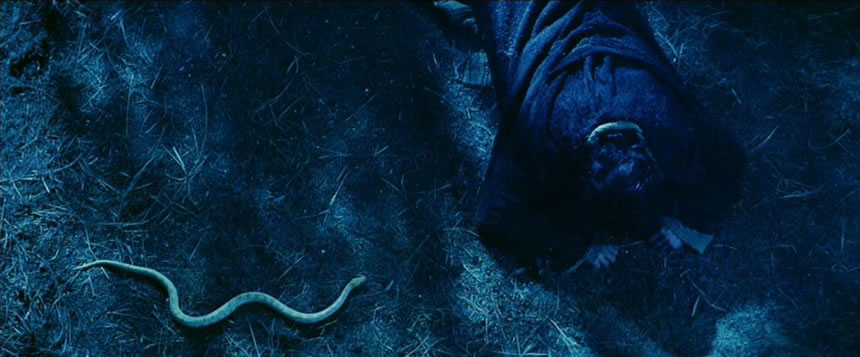
\includegraphics[width=0.8\linewidth]{passion}
	\caption{Screen shot of \textit{The Passion}, Jesus is fragile and being lured by Satan (the snake)}
	\label{fig:passoin}
\end{figure}

And even Jesus Christ, as a half-person-half-god, hidden his own person side when spreading parable but act like a God at this time. He only shows fear and could be tempted when he is alone inside the forest [John 6:26-31 NIV]. But his mundane and vulnerable ego fade away and turn back to a God look once he became Jesus in people's eyes. \textbf{When Jesus is disseminating, he is God, not himself}.

To draw a partial conclusion, the actor of involuntary communication, but whoever it is, the speaker themself (ego) is not speaking.

\section{"Who am I speaking to"}

At the first glance, the answer to most evident question "Who am I speaking to" is "nobody". It would be proper to interpret the Metamorphosis as a storyteller's mind telling stories for himself, and the external listener is nobody. But there is a better answer.   

Compared with Ovid, Socrates is obviously a more popular type. In modern age Socrates could be those who enjoy party and night club, while Ovid is so lonely that he could only tell stories to himself. For this sense, it could be simply interpreted as an emotional exit.

But in psychology term, a conversation without listener is hazardous. This emotional burst could trigger a defense mechanism named \textit{Rationalization}~\cite{simon2009understanding}. In general term, whenever people are forced or involuntarily to behave irrationally, an explanation would be triggered, and force out a rationale. This rationale could be a false image that \textit{"I am creating epic and writing for the world"}, \textit{"I have an imaginary friend"} or \textit{"I am guided by angle"}. Whatever person they assume they are speaking to, \textit{Speaking into the air} is forbidden.

\begin{figure}
	\centering
	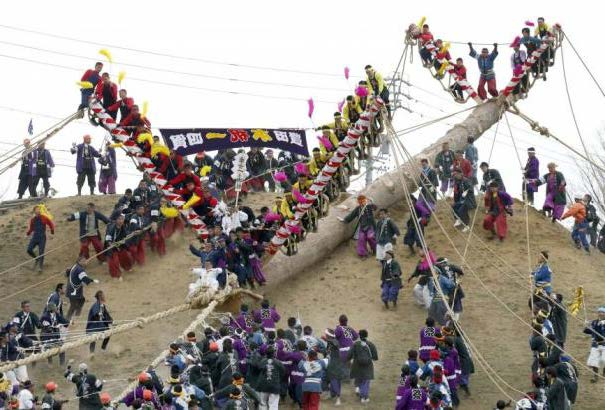
\includegraphics[width=0.6\linewidth]{ritual}
	\caption{Onbashira Festival, “Onbashira” basically means “sacred pillar”, those pillars could weight 10 tons }
	\label{fig:pillar}
\end{figure}

A good example of application of \textit{Rationalization} in anthropology is the Onbashira festival in Japan. Every 6 year Japanese people would erect wooden pillar/log by human power ~\ref{fig:pillar}, which could be 17 to 19 meters high and very dangerous. Scholars argue that this behaviour used to be vital for ancient construction but meaningless now, and due to the tremendous effort people have devoted in, nobody could afford the trauma of admitting it to be meaningless ~\cite{csapo2005theories}. So, it is kept as a traditional ritual till present. 

In this way, a dialogue is "speak to other", dissemination is more of "speak to self" as a mean of healing when "other people" is diluted and fades away. But only after \textbf{the real listener fades away, imaginary listeners of this conversation grow out}. Due to this fact, the listeners of conversation are constructed in a defensive condition, and are potentially more evil than the listeners in a conversation.

% speaking for/to, is a defensive mechnaism, naturally self means speaking against other

One essential point to note is that these \textbf{dissemination looks aggressive but is defensive inside}. Based on the defensiveness of those involuntary conversations, it is not hard to answer that those people are speaking not to but against the potential trauma that could be brought by other. For those involuntary speakers, the audiences are born to be adversary, enemy or heretic instead of equal person to communicate with. They are not speaking to other, they are speaking to the conceptually harmful "other".

An interesting fact could be observed is that during the course of Jesus Christ, a few people joined him into the collective Christianity self, other successfully crossed him, became the conceptual \textit{big Other}, a sign of radical alterity could not be persuaded or conquered. This fact converge to the "efficiency" problem of parable~\cite{peters2012speaking} proposed by Peter, as \textit{"The parable of the sower"};

\begin{figure}
	\centering
	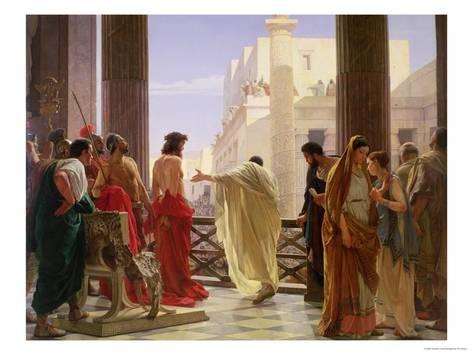
\includegraphics[width=0.8\linewidth]{ecce_homo}
	\caption{The famous "Ecce Homo" scene when the Roman governor attempted to save Jesus Christ from angry people}
	\label{fig:eccehomo}
\end{figure}

The normal dialogue that listeners either join tightly together or passionate to cross the speaker is rare. As Socrates is able to persuade other, but Christ could not persuade the conceptual other. The same thing is Socrates could only persuade other and could not move other so much that they virtually abandoned the individual self to join into a collective, big self. Besides, compared with the deliberate murder of Socrates, the cross of Jesus Christ is more similar to a radically irrational riot. For Christ and Christians proposing parable and compiling Bible is more similar to speaking to themselves, speaking internally. But the special effect of this psychoanalytical defensive murmuring is regarding other not as listeners but natural born enemies. (That is why it takes years for Jesus to collect disciples, but take thousands of years to "move and forgive" heretic)

%analogy to the history of christ when bible is compiled

And in the real world, this defensiveness goes according to the history of early stage Christianity, especially when the new Testament is accumulated ~\cite{warfield1948inspiration}. Jesus himself is the archetype of martyr, his disciples and thousands of believers follows him. It is fine to say that the early stage Christians are standing defensively against the world around, while passionately preaching their ideas at the same time. It is because the collective self is speaking for Christians, and it is taking a defensive posture.

So, speaking of Christians, if the collective self of Christian is a person, she/he would definitely take a defensive position. A historical impulse is accumulating with person desire, composing the specialness of this form of dissemination. 

\section{Conclusion}

There might be a tighter and more obvious connection between Socrates's dialogue and Gospels's dissemination, at least more obvious than the analogy between Eros and love: a dialogue happens between people and other people, a dissemination happens when people are not controlled by self, and the pose is against \textit{Other}, which functions as a defense or forecast towards possible traumatic. 

For the case of Christian, the believers are giving up their egos to merge into a collective ego. And this ego has a historical reason to be defensive. This better reveals the Bible without taken it as absolute truth and explains the feverish behind a "indifference attitude". 

\bibliographystyle{plain}
\bibliography{ref}


\end{document}


